\documentclass[10pt,a4paper]{report}
\usepackage[utf8]{inputenc}
\usepackage{amsmath}
\usepackage{amsfonts}
\usepackage{amssymb}
\usepackage{graphicx}
\usepackage{lmodern}
\usepackage[left=2cm,right=2cm,top=2cm,bottom=2cm]{geometry}
\begin{document}

\section{Setting up the problem}
Finite element solution of 
\begin{equation}\label{sim}
u^{\prime\prime} = 1\quad; u(0) = u^{\prime}(1)= 0
\end{equation}
and 
\begin{equation}\label{nosim}
u^{\prime\prime} = 1\quad; u(0) = u(1)= 0
\end{equation}
with 
\begin{equation}
V = \left\lbrace\sin\left( \frac{(i+1)\pi x}{2}\right)\right\rbrace; \quad i = 1,..,N
\end{equation}
\begin{equation}
V = \left\lbrace\sin( (i+1)\pi x)\right\rbrace; \quad i = 1,..,N
\end{equation}
applied to \ref{sim} and \ref{nosim} respectively.
The variational formulation or weak formulation of \ref{sim} and \ref{nosim} read:\\
find $u\in  V$ such that
\begin{equation}\label{var}
-\int_{0}^{1} u^{\prime} v^{\prime} \mathrm{d}x = \int_{0}^{1} v \mathrm{d}x
\quad \forall v\in V
\end{equation}

Using the Galerkin method let $u,v \in V$ be the trial function and the test function given by
\begin{equation}
u = \sum{c_{j}\varphi_{j}}
\end{equation}

\begin{equation}
v = \varphi_{i}
\end{equation}
Inserting the expression of $u$ and $v$ into \ref{var} gives
\begin{equation}
-\left(\int_{0}^{1} \varphi_{j}^{\prime} \varphi_{i}^{\prime} \mathrm{d}x\right)\sum{c_{j}} =\int_{0}^{1} \varphi_{j} \mathrm{d}x
\end{equation}
where 
\begin{equation}
A_{j,i} = -\int_{0}^{1} \varphi_{j}^{\prime} \varphi_{i}^{\prime} \mathrm{d}x
\end{equation}

\begin{equation}
b_{i} = \int_{0}^{1} \varphi_{j} \mathrm{d}x
\end{equation}
and the coefficient $c_{j}$ are solution of 
\begin{equation}
Ac = b
\end{equation}
\section{Solution of computation result}
for $N= 0$ and $x = 1$ the numerical solution of \ref{sim} and the analytical solution 
\begin{equation}
u(x) = -\frac{1}{2}x+x
\end{equation}
gives $-0.516024550931$ and $-0.5$ respectively. For verification see file $cable-sin.py$. figure \ref{fi} shows the variation of $\frac{c_{j}}{c_{j-1}}$ with $N$.
\begin{figure}[h!]\label{fi}
  \centering
    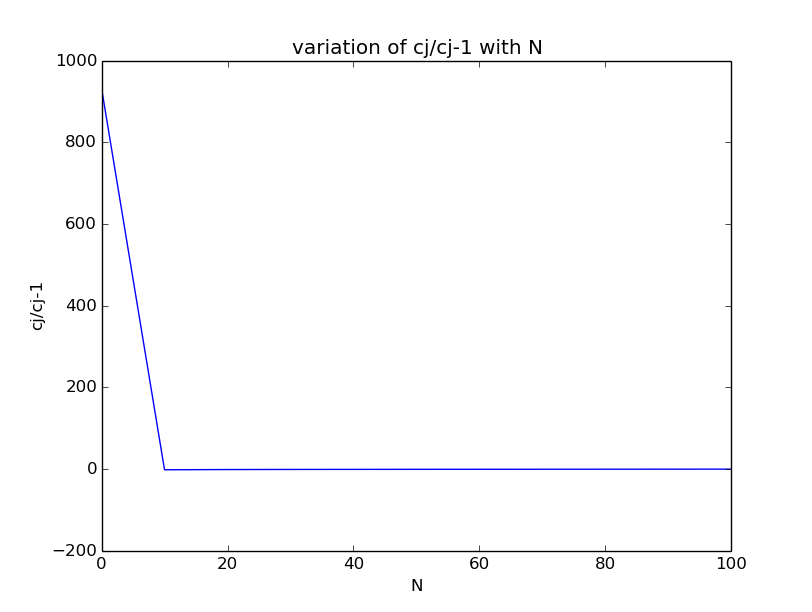
\includegraphics[width=0.5\textwidth]{p1.png}
\end{figure}
The numerical solution of \ref{sim} at $x=1$ and the numerical solution of \ref{nosim} at $x = 0.5$ gives the same result $-0.516024550931$. for verification see file $cable-sin.py$

\end{document}